\chapter{Branch prediction techniques}
As stated throughout the previous chapter, as well as in equation \eqref{eq:pipe_cpi}, in order to avoid stalls caused by control hazards and to ensure a steady flow of instructions to issue to the execution stages, one of the most important features of almost any modern high-performance processor is branch prediction. As seen for the multiple-issue paradigm, branch prediction too can be implemented at compile time or at run time, leading to two separate families of techniques, known as \emph{static} and \emph{dynamic} branch prediction.

The overall performance of a certain branch prediction technique can be essentially traced back to two factors:
\begin{itemize}
  \item \textbf{Accuracy}: that is the percentage of correctly predicted branch instructions. This figure depends only on the type of branch predictor used.
  \item \textbf{Misprediction penalty}: the CPU time lost in executing wrong path instructions in case of an incorrect prediction. This parameter is determined by the architecture of the processor and not by the branch predictor.
\end{itemize}

\section{Static branch prediction}
In static branch prediction, the action to be taken for each branch instruction is determined solely by the compiler and is then fixed at execution time. A number of static techniques exists \cite{smith98}:
\begin{itemize}
  \item Predict always taken (not taken): the accuracy of this method depends greatly on the \emph{program sensitivity} to the number of taken (not taken) branches, so results may vary according to the algorithm, the programmer and the compiler.
  \item Predict branches with certain opcodes as taken or not taken: as in \cite{smith98}, this technique gives better results than the previous one but only if the predictions are tailored to the benchmark algorithm.
  \item Predict backward branches (to lower \acp{PC}) as taken and forward branches as not taken: this strategy exploits the fact that in loops that iterate a large number of times, the condition is checked at the end of the body and so produces a backward branch if true. This can however introduce some delay needed to compute whether the target of the branch is higher or lower than the current \ac{PC}.
  \item Delayed branch \cite{gross82}: this is not actually a prediction technique, but a way to reduce the branch penalty, with the compiler scheduling (usually) one instruction that would be executed regardless of the branch outcome in a so called \emph{delay slot} which masks the delay of a single cycle stall in simple pipelines. In more complex \ooo pipelines, however, this can have harmful side effects, as mentioned in section \ref{sec:isas}.
\end{itemize}

Static prediction techniques have the advantage of adding no hardware complexity whatsoever by relying only on software technology, but on the other hand struggle to achieve satisfactory accuracy. For this reason, nowadays, they are used only in application specific processors or as an assist to more complex and performing dynamic techniques.

\section{Dynamic branch prediction}\label{sec:dynbp}
Dynamic strategies rely on the other hand on dedicated hardware to make predictions based on the actual run-time past behavior of branches. The general scheme of a dynamic branch predictor is shown in figure \ref{fig:bpfeedback}.
\begin{figure}[hbtp]
  \centering
  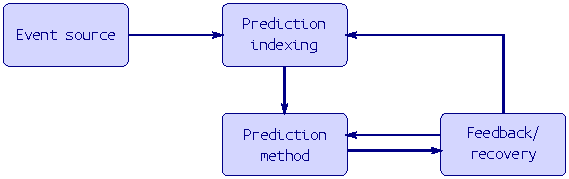
\includegraphics[width=0.8\textwidth]{img/bpfeedback.pdf}
  \caption{General dynamic branch predictor scheme}
  \label{fig:bpfeedback}
\end{figure}
An event source, that is the actual branch instruction, indexes a table with information about the past behavior of that branch (\emph{local history}) or of all previous branches (\emph{global history}). The information read from that table is used to make the prediction and finally, when the real outcome of the branch is resolved, the tables and the prediction method are updated, taking countermeasures in case of misprediction. It is effectively a feedback control system.

\subsection{Basic predictor structures}
The most basic dynamic predictor consists of a table of $2^k$ entries (flip-flops), called \ac{BHT}, addressed using $k$ bits from the branch \ac{PC}, that stores a single bit at each location to predict if the branch will be taken (value 1) or not taken (value 0). When the branch outcome is resolved, the table is updated so that it always predicts the direction that the branch took the last time. Figure \ref{fig:one-level-bp} shows this scheme.
\begin{figure}[hbtp]
  \centering
  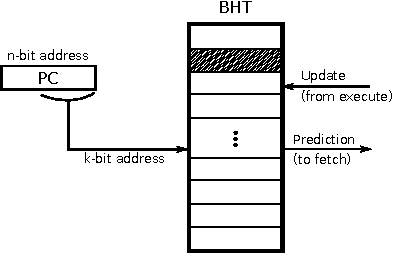
\includegraphics[width=0.8\textwidth]{img/one-level-bp.pdf}
  \caption[One-level branch predictor]{One-level branch predictor\footnotemark}
  \label{fig:one-level-bp}
\end{figure}
\footnotetext{Edited from \url{https://commons.wikimedia.org/wiki/File:Two-level_branch_prediction.svg} under the license \href{https://creativecommons.org/licenses/by-sa/3.0/deed.en}{Attribution-Share Alike 3.0 Unported}}

This one-bit model is however quite weak, especially with nested loops, as the inner loop is mispredicted twice: at the last iteration when exiting and at the next first iteration when entering again.

This predictor can be improved by introducing some hysteresis in the system using two bits instead of one. This way, the \ac{BHT} is composed by 2-bit entries that work as saturating counters, with their value incremented saturating at 3 every time the branch is taken and decremented saturating at 0 when the branch is not taken. The most significant bit of the counter provides the prediction, that changes only after two consecutive mispredictions.
\begin{figure}[hbt]
  \centering
  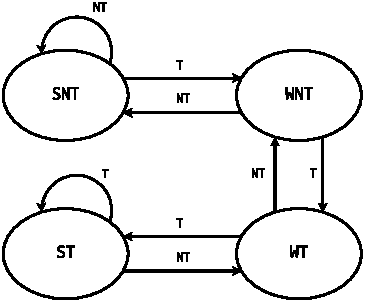
\includegraphics[scale=1.5]{img/c2b.pdf}
  \caption{2-bit counter FSM}
  \label{fig:c2b}
\end{figure}
These 2-bit counters are nothing more than simple state machines, that work as illustrated in \cref{fig:c2b}. \Cref{tab:c2b} shows the list of the counter states and their description.

\begin{table}[hbt]
  \centering
  \begin{tabular}{lll}
    \toprule
    \textbf{State}            & \textbf{Counter value}  & \textbf{Prediction} \\ \midrule
    Strongly not taken (SNT)  & 00                      & Not taken \\
    Weakly not taken (WNT)    & 01                      & Not taken \\
    Weakly taken (WT)         & 10                      & Taken     \\
    Strongly taken (ST)       & 11                      & Taken     \\
    \bottomrule
  \end{tabular}
  \caption{2-bit counter state description}
  \label{tab:c2b}
\end{table}

These designs, known as \emph{one-level} or \emph{bimodal} predictors, could be extended to $n$-bit saturating counters, but solutions with more than two bits are rarely employed, because the size of the table is the actual limiting factor, given that, by using only a subset of \ac{PC} bits, multiple branches could index the same \ac{BHT} entry, thus producing \emph{aliasing} issues.

\subsection{Two-level branch predictors}\label{sec:twolevelbp}
An improvement over the simple predictors of the previous section comes from the concept of \emph{correlation} between branches. Consider for example the following code:
\begin{lstlisting}[language=C]
  if (x)        // branch 1
      a = 0;
  if (y)        // branch 2
      b = 0;
  if (a != b)   // branch 3
      ...
\end{lstlisting}
If the first two branches are taken, then the third one will be not taken for sure, which means that these three branches are deterministically correlated.

A design that exploits such correlations was first proposed in \cite{yeh91} and it is called \emph{two-level predictor}, shown in figure \ref{fig:two-level-bp}. It features an $k$-bit \ac{BHT} shift register storing the outcome of the last $k$ executed branches (first level), pointing to a \ac{PHT} (second level) which stores $2^k$ 2-bit counters, one for each \ac{BHT} pattern combination.
\begin{figure}[hbtp]
  \centering
  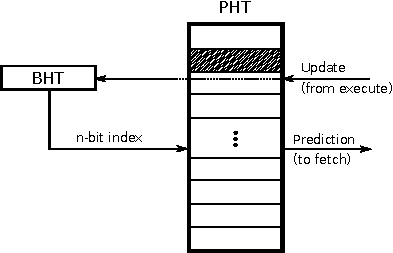
\includegraphics[width=0.8\textwidth]{img/two-level-bp.pdf}
  \caption[Two-level branch predictor]{Two-level branch predictor\footnotemark}
  \label{fig:two-level-bp}
\end{figure}
\footnotetext{Taken from \url{https://commons.wikimedia.org/wiki/File:Two-level_branch_prediction.svg} under the license \href{https://creativecommons.org/licenses/by-sa/3.0/deed.en}{Attribution-Share Alike 3.0 Unported}}
In the example above, the two-level predictor would successfully predict as not taken the third branch if the global history stored in the \ac{BHT} indicated that the previous two branches were taken.

This scheme, however, has lost the \emph{local} information about the current branch instruction, relying only on the global history of branches for the prediction. Thus, nine variants were proposed \cite{yeh93} that exploit either one or both the local and global information (figure \ref{fig:yehvariations}), by storing, for instance, multiple \acp{BHT} indexed by the branch address.

\begin{figure}[hbtp]
  \centering
  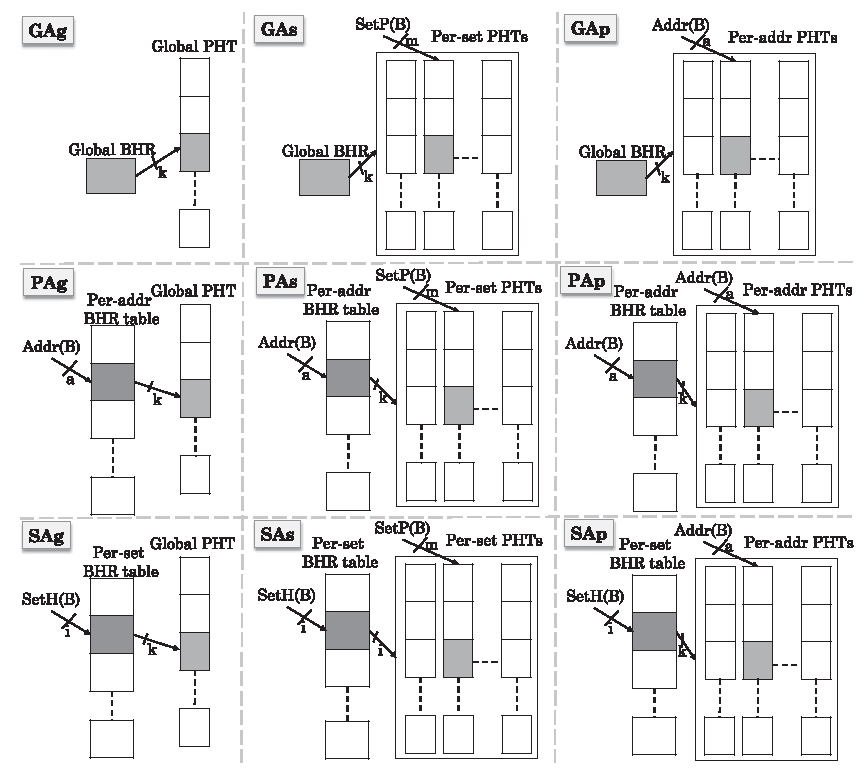
\includegraphics[width=\textwidth]{img/yehvariations.pdf}
  \caption{Two-level predictor variations \cite{mittal19}}
  \label{fig:yehvariations}
\end{figure}

\pagebreak
\section{State-of-the-art branch predictors}
Building on the schemes described in the previous sections developed in the 90s, nowadays modern high-performance processors use very advanced design for branch predictors, that even occupy a significant area on the chip die. Two main classes of state-of-the-art branch predictors are used today: \emph{\acs{TAGE}-based} predictors and \emph{perceptron-based} predictors.

\subsection{\acl{TAGE} predictor}
\acf{TAGE} predictors \cite{seznec06} use a series of global predictors indexed with histories of different length, like in the scheme shown in figure \ref{fig:tage}.
\begin{figure}[hbtp]
  \centering
  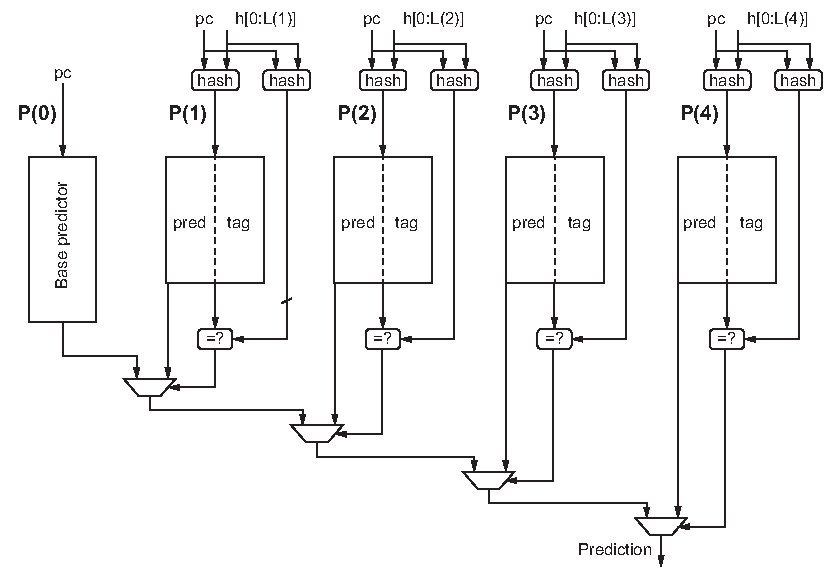
\includegraphics[width=\textwidth]{img/tage.pdf}
  \caption{\ac{TAGE} predictor \cite[p.~188]{hennessy17}}
  \label{fig:tage}
\end{figure}
The base predictor can be as simple as a basic bimodal predictor, while the others are variable-length two-level predictors that combine local and global branch information by hashing part of the branch \ac{PC} with the \acp{BHT}.

This predictor uses \emph{tagging} to avoid aliasing by saving a subset of the bits of the \ac{PC} not used for indexing in a dedicated field in the \ac{PHT}. All the predictors are accessed simultaneously and if more than one two-level predictors have a match between the branch address and the tag, then the prediction coming from the one with the longest global history is selected. If no two-level predictor hits, then the base predictor is used as a fallback.

Variants of this \ac{TAGE} predictor have been shown to win annual branch prediction competitions without needing too much memory size \cite[p.~189]{hennessy17} and are present in many high-end CPUs.

\subsection{Perceptron predictor}
These kinds of predictor take a completely different approach to the problem with respect to previously analyzed designs. The idea is based around the concept of the \emph{perceptron} \cite{jimenez01}, a single-layer artificial neuron, whose structure is shown in figure \ref{fig:perceptron}.
\begin{figure}[hbtp]
  \centering
  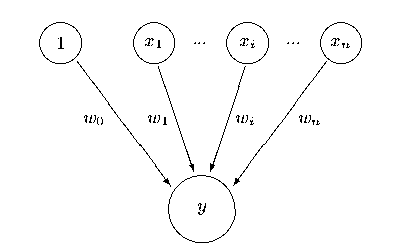
\includegraphics[width=.5\textwidth]{img/perceptron.pdf}
  \caption{Perceptron}
  \label{fig:perceptron}
\end{figure}
The perceptron receives a certain number of inputs $x_1 \ldots x_n$, that in the case of branch prediction correspond to the entries of the global history register (the previous outcomes), and computes the output $y$ as a weighted sum of its inputs:
\begin{equation*}
  y = w_0 + \sum_{i=1}^n x_i w_i
\end{equation*}
If the output turns out to be non-negative, then the branch is predicted as taken, otherwise as not taken.

The weights express the degree of correlation between the current and previous branches, specifically weight $w_i$ indicates how much the current branch is biased toward the result of the last-but-$i$ branch. The input corresponding to weight $w_0$ is always 1, to indicate the intrinsic bias of the current branch (if it is more likely to be taken or not regardless of previous history). These weights are updated with a training algorithm that is executed every time a new branch resolution arrives.

The structure of the complete perceptron predictor is shown in figure \ref{fig:perceptron-bp} and features a table of perceptrons indexed by the branch address, a block that computes the prediction starting from the selected perceptron and the global history and a training unit dedicated to updating the weights upon a new actual branch result.
\begin{figure}[hbt]
  \centering
  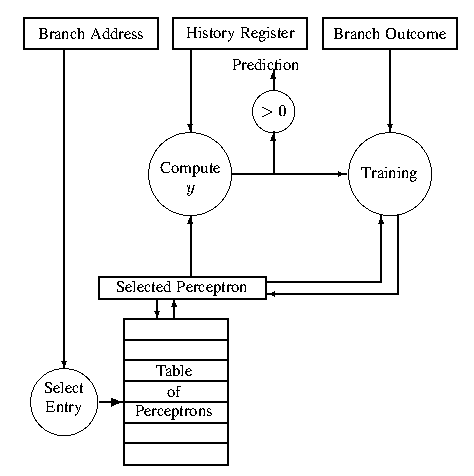
\includegraphics[width=.8\textwidth]{img/perceptron-bp.pdf}
  \caption{Perceptron-based branch predictor}
  \label{fig:perceptron-bp}
\end{figure}

Research \cite{jimenez01} has shown that this new approach offers complementary strengths to the previous ones and so that an optimal solution is developing a hybrid predictor between the two. At the present time, high-end processors for both desktop and mobile make use of some kind of perceptron-based prediction network, such as the AMD Ryzen and Samsung Exynos families.